\documentclass{../exhibit}

\title{Coin Puzzles}

%% Font
\usepackage{imfellEnglish}
\usepackage[T1]{fontenc}
\raggedright

\usepackage{background}

\backgroundsetup{
scale=1,
color=black,
opacity=0.4,
angle=0,
contents={%
  \includegraphics[height=\paperheight]{mapBackground.jpg}%%https://upload.wikimedia.org/wikipedia/commons/8/81/Nautical_chart_of_the_West_Indies_1797.jpg
  }%
}




%% For the context
%% https://tex.stackexchange.com/questions/86150/torn-page-effect/86151#86151
\usepackage{tikz}
\usetikzlibrary{decorations.pathmorphing}
\definecolor{paper}{RGB}{239,227,157}





\renewcommand{\maketitle}{ %
  \begin{center}
    \scalebox{8}{\thetitle}
  \end{center}
  
\begin{tabular*}{\textwidth}{c @{\extracolsep{\fill}} c}  
\resizebox{4in}{!}{\begin{minipage}[b]{3in}\huge\directions\end{minipage}} &
  \resizebox{4in}{!}{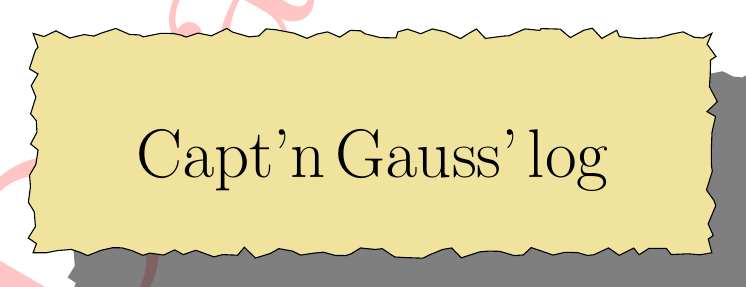
\begin{tikzpicture}[pencildraw/.style={ %
    decorate,
    decoration={random steps,segment length=4pt,amplitude=2pt}
    } %
]
\node[
preaction={fill=black,opacity=.5,transform canvas={xshift=.5cm,yshift=-.5cm}},
pencildraw,draw,fill=paper,text width=3in,inner sep=.5cm] 
{\begin{center}\Huge Capt'n Gauss' log \end{center}\vspace{.7cm} {\huge\context}};
\end{tikzpicture}}

\end{tabular*}

\vfill

\includegraphics[width=3in]{logoPirate.png}\hfill \includegraphics[width=2in]{bammLogo.png}


}


\begin{document}

\begin{context}
  Coins have a value that's well known,
  \\[1cm]
  But puzzles be worth more than gold!
\end{context}

\begin{directions}
  Move the coins from one side to the other with the following rules:
\begin{itemize}
\item The gold can only move in one direction. The silvers move in the opposite direction.
\item Each coin can only move to the next adjacent empty square.
\item Each coin can jump only one coin at a time to land into an empty
  square.
\end{itemize}
\end{directions}


\begin{example}
  Make this:
  \begin{center}
    \begin{tikzpicture}[x=1in, y=1in]
      \foreach \x in {1,...,7} {
        \draw[line width=3pt] (\x-1,0) rectangle (\x ,1);
      }
      \foreach \x in {1,...,3} {
       \node at (\x-.5,.5) {\includegraphics[scale=.6]{silvercoin.png}};
      }
      \foreach \x in {5,...,7} {
       \node at (\x-.5,.5) {\includegraphics[scale=.6]{goldcoin.png}};
      }
\end{tikzpicture}
  \end{center}
Into this:
  \begin{center}
    \begin{tikzpicture}[x=1in, y=1in]
      \foreach \x in {1,...,7} {
        \draw[line width=3pt] (\x-1,0) rectangle (\x ,1);
      }
      \foreach \x in {1,...,3} {
       \node at (\x-.5,.5) {\includegraphics[scale=.6]{goldcoin.png}};
      }
      \foreach \x in {5,...,7} {
       \node at (\x-.5,.5) {\includegraphics[scale=.6]{silvercoin.png}};
      }
\end{tikzpicture}
  \end{center}
\end{example}


\begin{mathConnections}
  https://bartsnapp.github.io/Math-Outreach-Exhibits/coinPuzzle/
\end{mathConnections}

\end{document}
